\documentclass[]{article}
\usepackage{amsmath}
\usepackage{amsfonts}
\usepackage{amssymb}
\usepackage[utf8]{inputenc}
\usepackage{graphicx}
\usepackage{geometry}
\usepackage{color}
\usepackage{siunitx} %\SI{44.9}{\celsius}
\usepackage[german]{babel}
\usepackage{fancyref}
%\usepackage{circuitikz} für Stromkreise
\long\def \/*#1*/{} %Kommentare mit \/* ---- */
\geometry{
	a4paper,
	left=25mm,
	right=25mm,
	top=25mm,
	bottom=25mm,
}
\pagenumbering{arabic}

\title{Messung der Dampfdruckkurve von Wasser}
\date{}
\author{Mate Farkas, Patrick Schillings}
\begin{document}
	
	\maketitle
	
	\tableofcontents
	
	\noindent\makebox[\linewidth]{\rule{\textwidth}{0.4pt}}
	
	\section{Versuchsziele}
	Ziel des Versuchs war es durch die Messung der Dampfdruckkurve von Wasser, also den Druck in Abhängigkeit von der Temperatur während der Abkühlphase bei festem Volumen, die molare Verdampfungsenthalpie von Wasser zu bestimmen. Der Dampfdruck ist ein Gleichgewichtsdruck, der sich einstellt, wenn sowohl die flüssige Phase, als auch die gasförmige Phase im Gleichgewicht sind bei hinreichender Größe des Volumens. Die molare Verdampfungsenthalpie ist die Wärme, die ein Mol Flüssigkeit aufnimmt, um in die Gasphase übergehen zu können, und wird auch latente Wärme genannt.
	\section{Theoretische Grundlagen}
	Hintergrund ist die Clausius-Clapeyron-Gleichung, die aus den ersten beiden Hauptsätzen der Thermodynamik folgt.\\
	Der erste Hauptsatz behandelt dabei die Energieerhaltung,
	\begin{equation}
	\Delta U =\Delta Q +\Delta W
	\label{e1}
	\end{equation}
	wobei $\Delta U $ für die Veränderung der inneren Energie, $\Delta Q$ für die zugeführte bzw. abgegebene Wärme und $\Delta W$ für die am System geleistete Arbeit steht.\\
	Der zweite beschreibt die Umwandelbarkeit von verschiedenen Energieformen ineinander, was oft mit Hilfe der Entropie formuliert wird:
	\begin{equation} 
	\Delta S=\frac{\Delta Q_{rev}}{T} \ge 0
	\label{e2}
	\end{equation}
	Daraus folgt mit \eqref{e1} für einen infinitesimalen Prozess entlang der Grenzkurve:
	\begin{equation} 
	\nu((C_{m2}-C_{m1})dT+\frac{d\Lambda}{dT}dT=dp(V_1-V_2)
	\label{e3} 
	\end{equation}
	wobei $V_1$ das Volumen des Gases, $V_2$ das der flüssigen Phase und $C$ die molare Wärmekapazität (zu den Massen $m_1$ und $m_2$) sind.
	Mit \eqref{e2} erhält man
	\begin{equation} 
	(C_{m2}-C_{m1})dT+\frac{d\Lambda}{dT}dT-\Lambda\frac{dT}{T}=0,
	\label{e4}
	\end{equation}
	was mit \eqref{e3} zur oben genannten Clausius-Clapeyron-Gleichung führt:
	\begin{equation} 
	\frac{dp}{dt}=\frac{\nu\Lambda}{T(V_1-V_2)} 
	\end{equation}
	Daraus kann man durch Integrieren einen Zusammenhang zwischen dem Druck p und der Temperatur T herauslesen, der über Naturkonstanten und die molare Verdampfungsenthalpie $\Lambda$ gegeben ist: 
	\begin{equation}
	\ln\left(\frac{p}{p_0}\right)=-\frac{\Lambda}{R}\left(\frac{1}{T}-\frac{1}{T_0}\right)
	\label{e6}
	\end{equation}
	Mit der idealen Gasgleichung $pV=\nu RT$ und der Gaskonstanten R.
	\section{Versuchsaufbau}
	Ein Rundkolben, der an einem Stativ befestigt ist, befindet sich über einem mit einem Laborheber in der Höhe einstellbaren Heizpilz. Der Kolben hat einen abgedichteten Einlass für den Temperatursensor und oben wird mit dichten Schläuchen ein Drucksensor (Absolutdrucksensor S (524065)) angebracht und ebenso die Zuleitung zu einem Dreiwegehahn gelegt, von dem ein weiteres Ende mit einer Handpumpe verbunden wird. Ein Ausgang ist mit der Umgebung verbunden (vgl. Abb. \ref{Aufbau}).
	\begin{figure}
		\begin{center}
			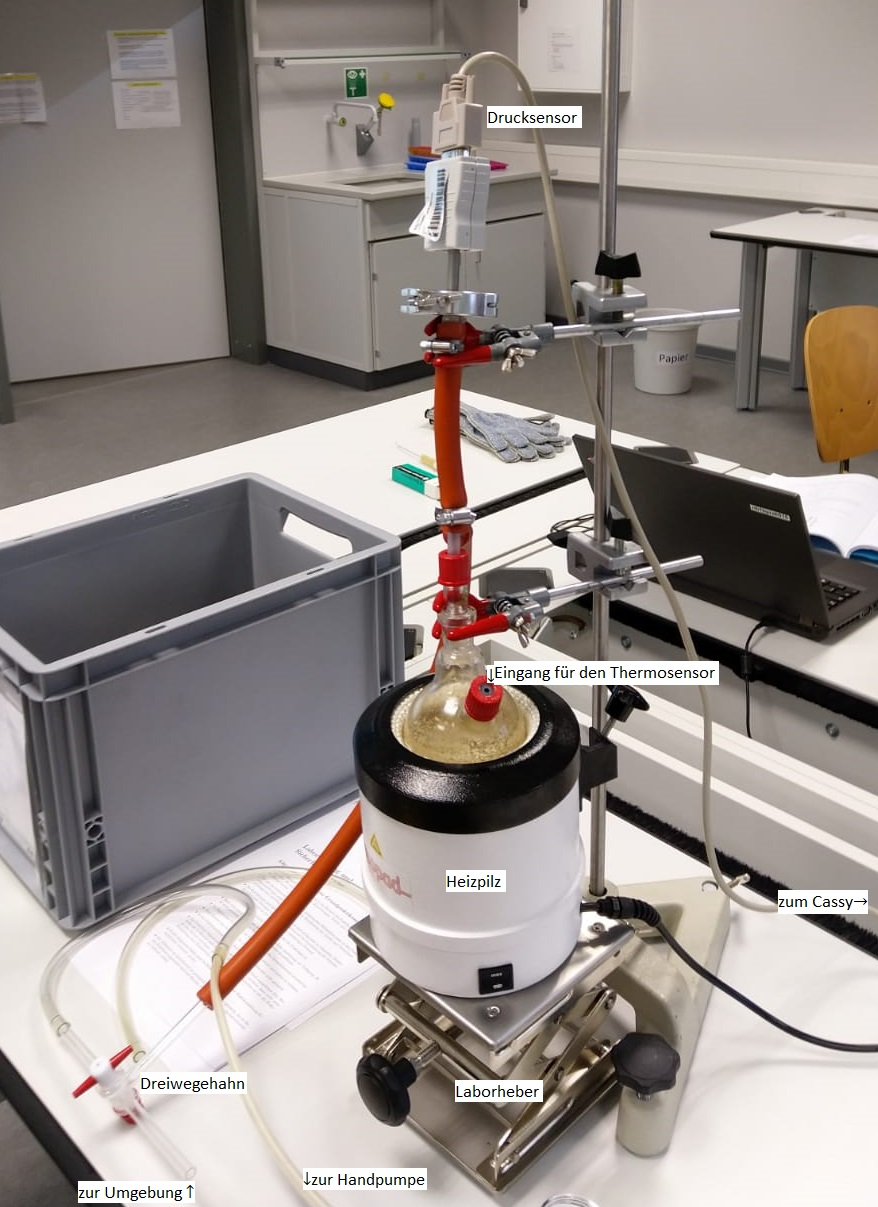
\includegraphics[scale=0.85]{Images/Aufbau.jpg}
			\caption{Der Versuchsaufbau}
			\label{Aufbau}
		\end{center}
	\end{figure}
	Ein Becherglas mit Eiswasser und ein Becherglas mit unbearbeitetem Wasser stehen bereit. Zur Datensammlung und Erstauswertung wird ein Cassy-System mit den zugehörigen Sensoren verwendet (vgl. Abb. \ref{Cassy}), wobei der Temperatursensor auf ein Intervall von \SI{-20}{\celsius} bis \SI{120}{\celsius} und der Drucksensor auf ein Intervall von \SI{0}{\hecto\pascal}-\SI{1500}{\hecto\pascal} eingestellt wurde.
	\begin{figure}
		\begin{center}
			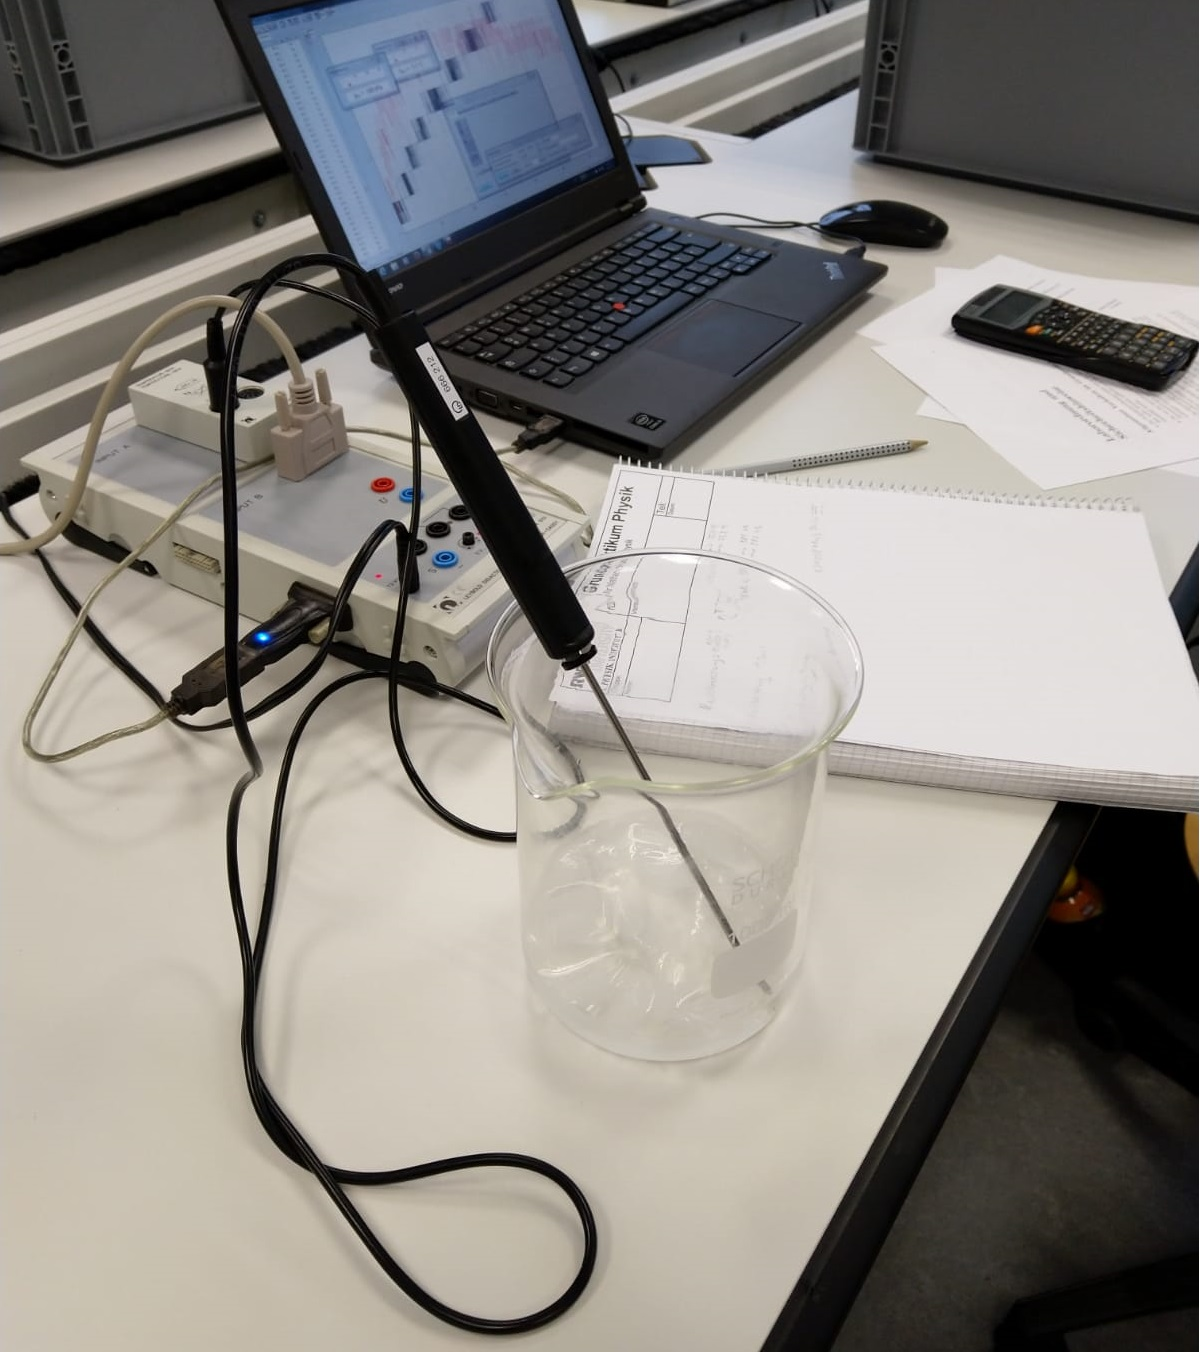
\includegraphics[scale=0.33]{Images/Cassy.jpg}
			\caption{Das verwendete Cassy-System samt Temperatur-Box und Druck-Input}
			\label{Cassy}
		\end{center}
	\end{figure}
	
	
	\section{Durchführung}
	\subsection{Rauschmessung}
	Bei Raumtemperatur und Umgebungsdruck findet eine 'Leerlauf'-Messung statt, um den statistischen Fehler der Messgeräte gut abschätzen zu können. Dabei wird ein kurzes Zeitintervall bei hoher Messrate ausgewertet. 
	Einstellungen: Messung alle 10ms, 16000 mal $\widehat{=}$ 3min
	
	\subsection {Kalibrierung des Thermosensors}  
	Die Temperatur in Eiswasser wird zunächst gemessen, deren theoretischer Wert \SI{0}{\celsius} ist. Dazu wird Eis mit ein wenig Wasser gemischt und gewartet, bis ein Temperaturausgleich stattgefunden hat, der, solange noch festes Eis vorhanden ist, bei \SI{0}{\celsius} sein sollte, und die 7s Ansprechzeit, die der Sensor nach Angaben des Herstellers hat, verstrichen ist. Später, wenn das Wasser siedet, wird noch dessen Siedetemperatur bestimmt, die \SI{100}{\celsius} sein sollte. Mit einem linearen Modell kann man nun $T_{real}(T_{gemessen})$ bestimmen.
	Einstellungen: Messung alle 100ms, insgesamt 3 Minuten lang.
	
	\subsection{Gasdichtigkeit}
	Um festzustellen, wie gasdicht der Aufbau ist, wird mit der Handpumpe im Kolben ein Unterdruck von etwa 190 hPa absolut erzeugt. Dann wird über einen Zeitraum von 10 Minuten der Druck gemessen, um hinterher mit Hilfe einer linearen Regression die Leckrate bestimmen zu können, die nicht höher als 0.2 mbar/min sein sollte, um zu gewährleisten, dass die gemessenen Druckwerte während der Hauptmessung nicht zu stark verfälscht werden. 
	Einstellungen: Messung alle 100 ms, insgesamt 3 Minuten lang.
	
	
	\subsection{Hauptmessung - Dampfdruckkurve}
	Durch den zuvor erzeugten Unterdruck kann über den Dreiwegehahn Wasser in den Rundkolben gesaugt werden, bis dieser etwa halb voll ist. Mit Hilfe des Heizpilzes wird das Wasser bei Kontakt zur Umgebung zum Kochen gebracht und so lange kochen gelassen, bis der entstehende Wasserdampf sämtliche Restluft aus dem Rundkolben gedrückt hat. Dies prüft man, indem man den Verbindungsschlauch zur Umgebung in ein Wasserbad hält. Der Wasserdampf kondensiert sofort, das heißt, solange Blasen aufsteigen, befindet sich noch Luft im Rundkolben, deren Partialdruck die Messung verfälschen würde. In dieser Zeit wird auch die Kalibrierung bei \SI{100}{\celsius} durchgeführt. Schließlich wird der Heizpilz schnell mit dem Laborheber heruntergefahren und die Messung des Dampfdrucks und der Gastemperatur gestartet. Später sollen die Ergebnisse p und T in der Form $\ln(p/p_0)$ gegen $1/T-1/T_0$ aufgetragen werden, um aus der Steigung des Graphen $\Lambda$ zu bestimmen.
	Einstellungen: Messung alle 100 ms, unbegrenzte Messdauer (Ende nach etwa einer Stunde)\\
	
	\subsection{Gasdichtigkeit 2}
	
	Nach der eigentlichen Versuchsdurchführung kann eine weitere Gasdichtigkeitsmessung wie 4.3. durchgeführt werden, um zu gewährleisten, dass sich die Leckrate am Aufbau nicht verändert hat. Diese entfällt aber bei uns, da keine Zeit mehr ist.
	
	\section{Auswertung}
	\subsection{Rauschmessung}
	Die Rauschmessung umfasst 3326 Datenpunkte, bei denen der Temperatursensor in Ruhe die als konstant angenommene Raumtemperatur gemessen hat, der Absolutdrucksensor zugleich den konstanten Umgebungsdruck. Dabei soll die Streuung der Werte um den Mittelwert erarbeitet werden, um den statistischen Fehler für alle folgenden Messungen abschätzen zu können.\\
	Die Ergebnisse sind wie folgt (Abb. \ref{RM_T_p}):\\
	\begin{figure}[h]
		\begin{center}
			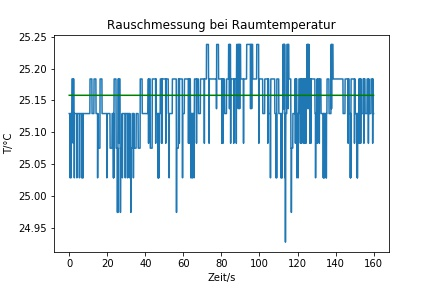
\includegraphics[scale=0.45]{Images/RauschmessungRT_T.jpg}
			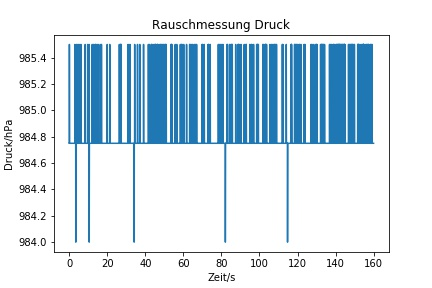
\includegraphics[scale=0.45]{Images/RauschmessungRT_p.jpg}
			\caption{Messergebnisse der Raumtemperatur-Rauschmessung}
			\label{RM_T_p}
		\end{center}
	\end{figure}\\
	Die Temperaturmessung ergab einen Mittelwert von etwa \SI{25.15797}{\celsius} mit einer Standardabweichung von \SI{0.04443}{\celsius}.  Daraus ergibt sich ein statistischer Fehler von \SI{0.00077}{\celsius} (vgl. Abb.\ref{RM_T_histo}).\\
	Die Druckmessung lieferte einen Mittelwert von \SI{984.7955}{\hecto \pascal} mit einer Standardabweichung von \SI{0.1838}{\hecto \pascal} und einem Fehler von \SI{0.0032}{\hecto \pascal} (vgl. Abb.\ref{RM_p_histo}).
	Systematische Fehler werden in dieser Messung nicht betrachtet, da hier nicht das Ergebnis interessant war, sondern die Standardabweichung. Diese wird im Folgenden benutzt werden, um eine genauere Fehlerabschätzung für den statistischen Fehler der Versuche zu bekommen, unter der Annahme, dass der Thermosensor stets gleich stark streut.
	\begin{figure}
		\begin{center}
			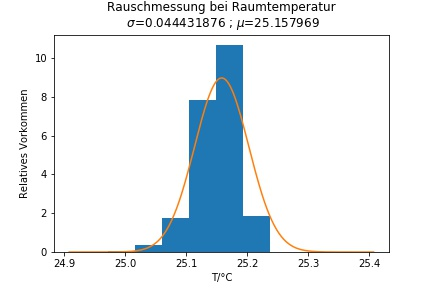
\includegraphics[scale=0.9]{Images/RauschmessungRT_T_histo.jpg}
			\caption{Histogramm der T-Rauschmessung}
			\label{RM_T_histo}
		\end{center}
	\end{figure}
	\begin{figure}
		\begin{center}
			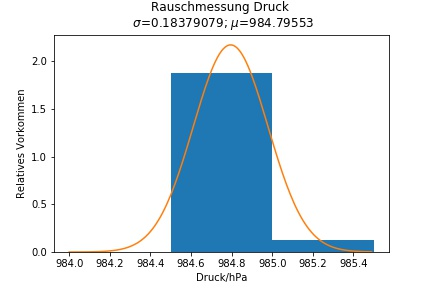
\includegraphics[scale=0.9]{Images/RauschmessungRT_p_histo.jpg}
			\caption{Histogramm der p-Rauschmessung}
			\label{RM_p_histo}
		\end{center}
	\end{figure}
	
	\subsection{Kalibrierung des Thermosensors}
	Zur Kalibrierung des Thermometers wurde die Temperatur bei theoretischen \SI{0}{\celsius} in Eiswasser und \SI{100}{\celsius} in siedenden Wasser bei Umgebungsdruck aufgezeichnet (vgl. Abb. \ref{K_Roh}).
	\begin{figure}
		\begin{center}
			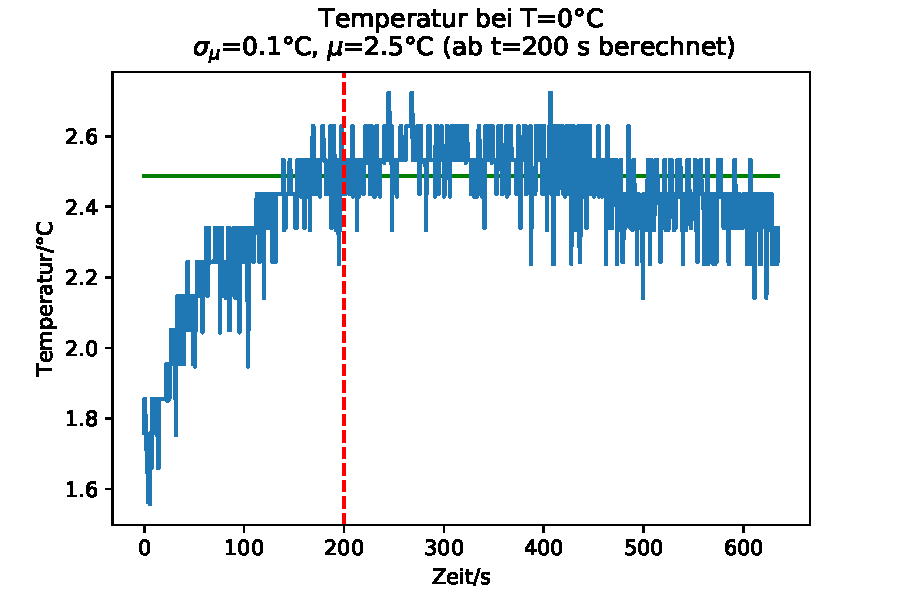
\includegraphics[scale=0.45]{Images/Kalib_T_0.pdf}
			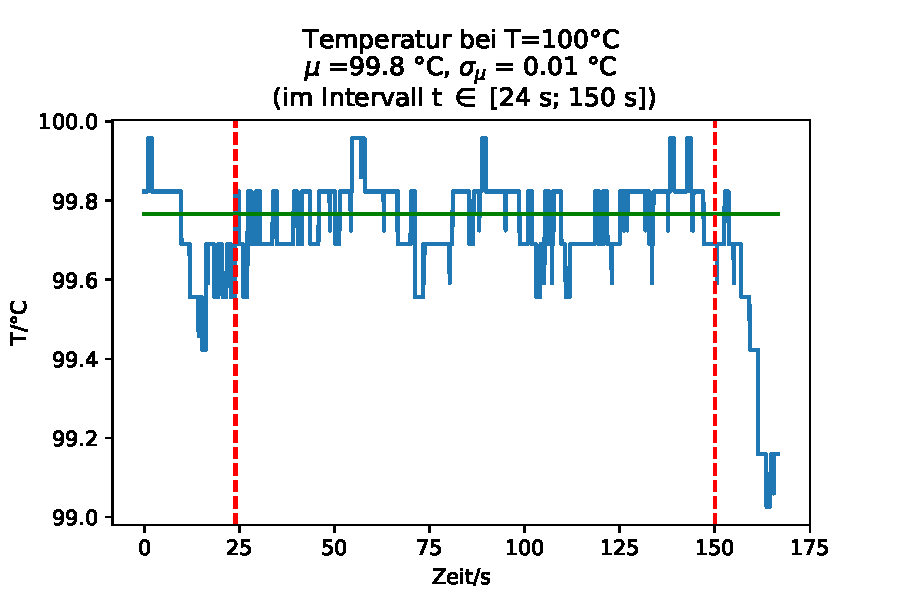
\includegraphics[scale=0.45]{Images/Kalib_T_100.pdf}
			\caption{Rohdaten und Histogramm der Kalibrierung in Eiswasser}
			\label{K_Roh}
		\end{center}
	\end{figure}
	Mit einem linearen Modell, dessen Unterstützungspunkt in der Mitte liegt, wird eine stabile Umrechnung von den gemessenen Werten zu den realen angestrebt: $T_{gem} = a*(T_{th}-50) + b + 50$ oder auf $T_{th}$ umgestellt $T_{th} = (T_{gem}-b-50)/a + 50$. \\
	
	In Eiswasser stellte sich ein Mittelwert von $T_0=\SI{2.4865}{\celsius} \pm \SI{0.0015}{\celsius} \pm \SI{0.2}{\celsius}$ ein, wobei der erste Fehler den statistischen Fehler als Standardabweichung der Rauschmessung geteilt durch die Wurzel aus der Anzahl der jetzt gemessenen Werte und der zweite den systematischen Fehler aus der Angabe des Herstellers des Thermosensors angibt.  (vgl. Abb. \ref{K_T0_histo})\\
	\begin{figure}
		\begin{center}
			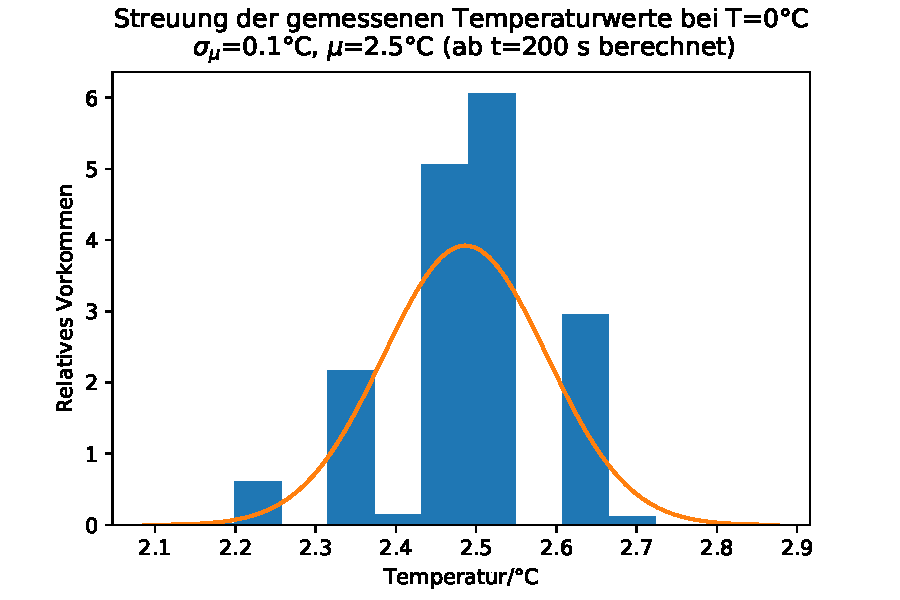
\includegraphics[scale=0.9]{Images/Kalib_T_0_histo.pdf}
			\caption{Histogramm der Kalibrierung in Eiswasser}
			\label{K_T0_histo}
		\end{center}
	\end{figure}
	Die Messung in siedendem Wasser ergab $T_{100}=\SI{99.766}{\celsius} \pm \SI{0.0025}{\celsius} \pm \SI{0.4}{\celsius}$. (vgl. Abb. \ref{K_T100_histo})\\
	\begin{figure}
		\begin{center}
			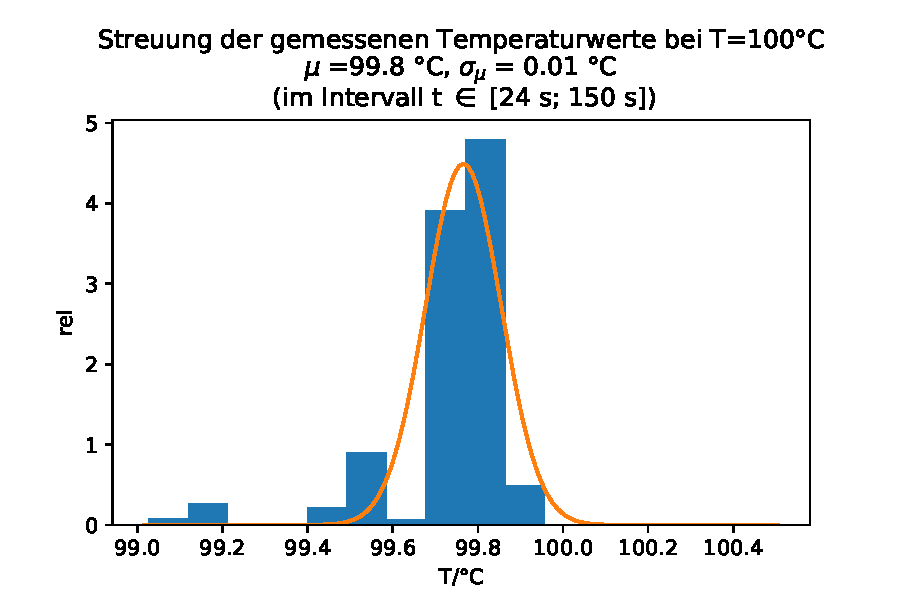
\includegraphics[scale=0.9]{Images/Kalib_T_histo_100}
			\caption{Histogramm der Kalibrierung in siedenden Wasser}
			\label{K_T100_histo}
		\end{center}
	\end{figure}
	Somit lautet die Umrechnung
	mit $a = 0.9728 \pm 0.0006 \pm 0.0045$
	und mit $b = \SI{1.13}{\celsius} \pm \SI{0.03}{\celsius} \pm \SI{0.22}{\celsius}$:
	\begin{equation}
	T_{th} = (T_{gem}-\SI{1.13}{\celsius}-\SI{50}{\celsius})/0.9728 + \SI{50}{\celsius}
	\label{Kalibrierung}
	\end{equation}
	Es ergibt sich zum Beispiel mit Fehlern aus der Gaußschen Fehlerfortpflanzung 	
	\begin{equation}
	\sigma_T = \sqrt{\left(\frac{T_gem-b-50 ^{\circ}C}{a^2}\right)^2 \cdot \sigma_a^2 +\left(\frac{\sigma_b}{a}\right)^2 + \left(\frac{\sigma_{Tgem}}{a}\right)^2}
	\end{equation}
	$T_{th}(T_{100}) = \SI{100.00}{\celsius} \pm  \SI{0.06}{\celsius} \pm \SI{0.52}{\celsius}$
	und $T_{th}(T_0) = \SI{0.00}{\celsius} \pm \SI{0.06}{\celsius} \pm \SI{0.38}{\celsius}$
	\\
	\subsection{Gasdichtigkeitsmessung}
	Die Gasdichtigkeitsmessung ist eine einfache Prüfung, ob die Druckwerte sich im Laufe der Messung nicht zu stark verändern werden.
	\begin{figure}
		\begin{center}
			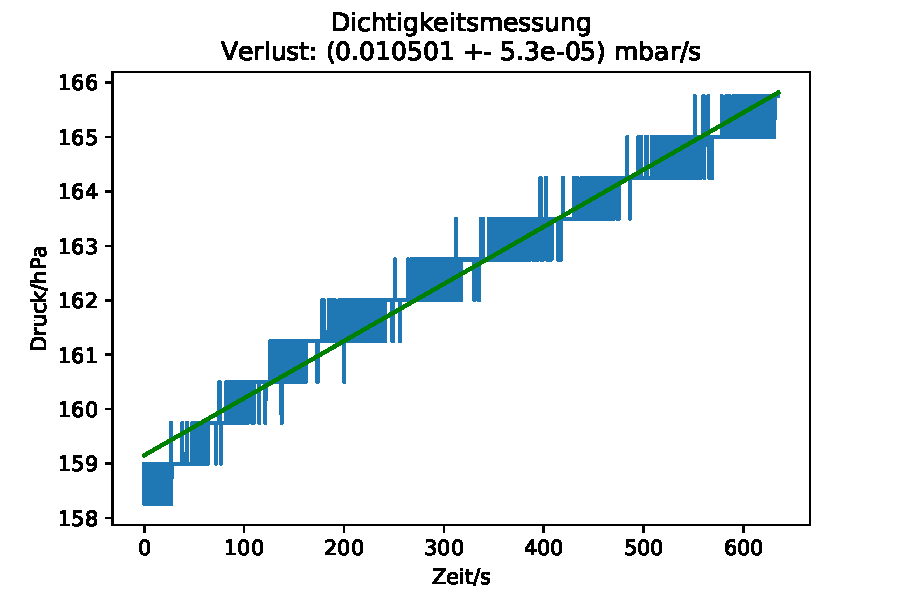
\includegraphics[scale=0.9]{Images/Kalib_Dichtigkeitsmessung.pdf}
			\caption{Verlauf der Dichtigkeitsmessung}
			\label{GD_data}
		\end{center}
	\end{figure}
	Die Ergebnisse waren wie in Abb. \ref{GD_data} dargestellt. \\
	Der Fehler auf jeden gemessenen Druckwert beträgt bedingt durch die Auflösefähigkeit des Absolutdrucksensors von $0.05\%$ auf den Wertebereich von \SI{1500}{\hecto \pascal} und die
	Standardabweichung aus der Rauschmessung $s^{2} = s^{2}_{Aufl\ddot{o}sung}+s^{2}_{Rausch} = \SI{0.60}{\hecto \pascal}$. 
	Eine lineare Regression der Form $p(t)=m*t+b$ ergibt $m = (0.010501 \pm 5.3*10^{-5})\SI{}{\hecto \pascal/ \second}$ und $b = (159.151 \pm 0.019)\SI{}{\hecto \pascal}$ mit einem ordentlichen $\chi ^{2}/N=1142.24 / 6346$. Das entspricht also einem Verlust von $60*(0.010501 \pm 5.3*10^{-5})\SI{}{\milli \bar / \minute}$ bei einem Innendruck von $162.483 \pm 0.025 \SI{}{\hecto \pascal} \approx 0.165*p_0$. Mit diesen Werten konnte weitergearbeitet werden.
	\subsection{Messung der Dampfdruckkurve}
	In der eigentlichen Hauptmessung wurden die Rohdaten aus Abb.\ref{DD_Roh} aufgezeichnet.\\
	\begin{figure}
		\begin{center}
			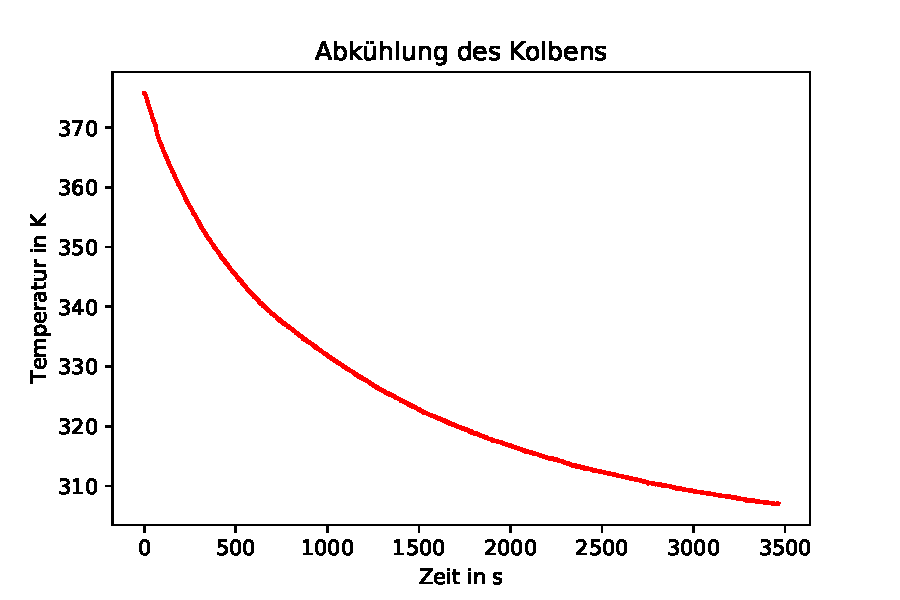
\includegraphics[scale=0.45]{Images/Dampfdruck_T.pdf}
			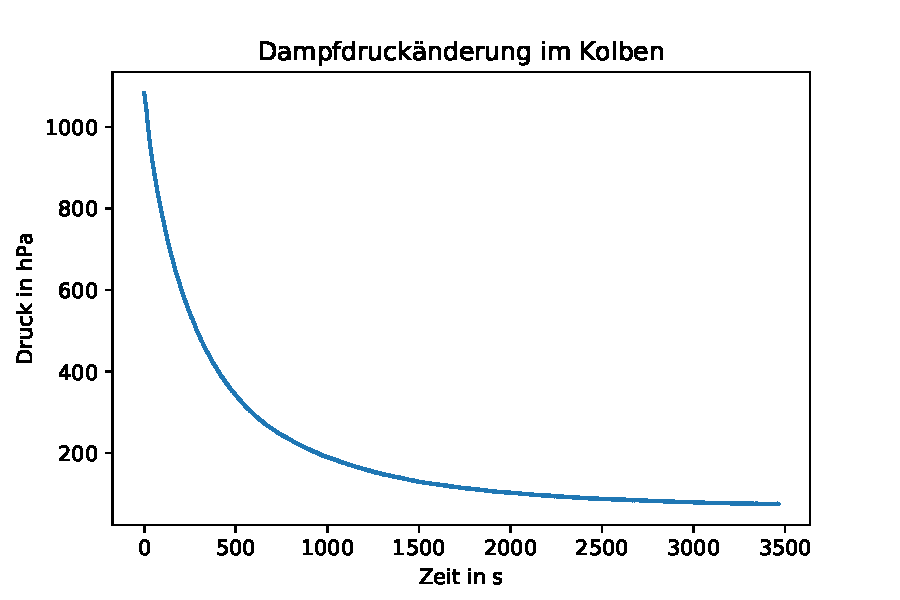
\includegraphics[scale=0.45]{Images/Dampfdruck_p.pdf}
			\caption{T und p während des Abkühlvorgangs}
			\label{DD_Roh}
		\end{center}
	\end{figure}
	Diese kann man nun in die Form $ln\frac{p}{p_0\\}$ und $\frac{1}{T} - \frac{1}{T_0}$ bringen, um mit ihnen und Gleichung \ref{e6} die molare Verdampfungsenthalpie zu bestimmen (vgl. Abb. \ref{DD_ln-1}). Dies geschieht durch eine lineare Regression. 
	\begin{figure}
		\begin{center}
			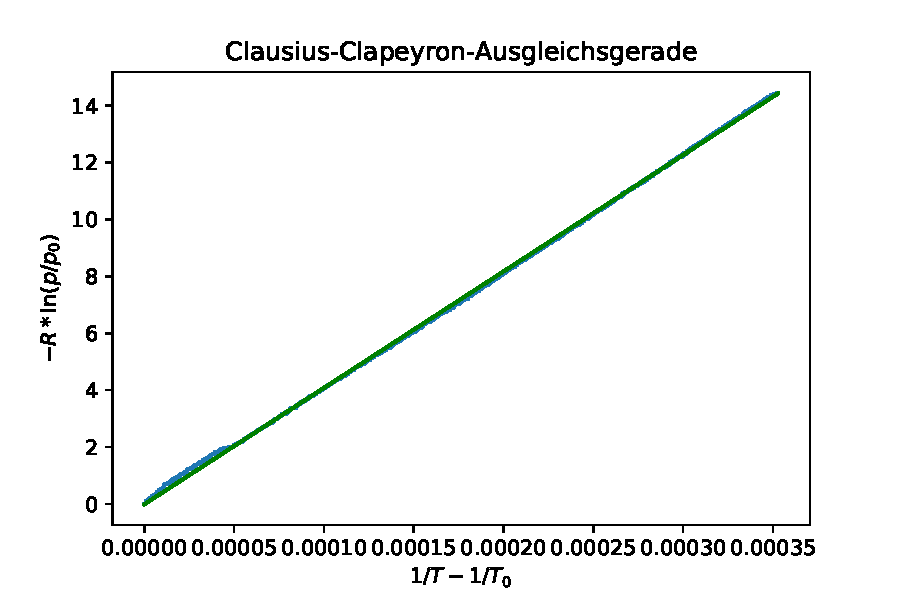
\includegraphics[scale=0.9]{Images/Dampfdruck_ln.pdf}
			\caption{$\ln(\frac{p}{p_0})$ gegen $\frac{1}{T} - \frac{1}{T_0}$}
			\label{DD_ln-1}
		\end{center}
	\end{figure}
	Die Fehler, die aus der Rauschmessung und den Geräten entstanden und durch die Kalibrierung bearbeitet wurden, werden dabei entsprechend der Fehlerfortpflanzung weitergetragen.
	\begin{equation}
	\text{Mit x} = \frac{1}{T} - \frac{1}{T_0}:
	\sigma_x = \sqrt{\left(\frac{\sigma_T}{T^2}\right)^2+\left(\frac{\sigma_{T_0}}{T_0^2}\right)^2}
	\end{equation}
	
	\begin{equation}
	\text{Mit y} = -R\ln\left(\frac{p}{p_0}\right):
	\sigma_y = R \sqrt{\left(\frac{\sigma_p}{p}\right)^2 +\left(\frac{\sigma_{p0}}{p_0}\right)^2 }
	\end{equation}
\\
	Um eine Tabelle von $\Lambda$ zu ermöglichen, wurden in Tausenderschritten die Werte der Enthalpie berechnet. Da man sowohl einen statistischen, als auch einen systematischen Fehler hat, muss diese Rechnung zweimal durchgeführt werden. Die resultierenden Endwerte werden nach dem Fehler gewichtet zusammengefügt 
	Die Abhängigkeit von $\Lambda$ von der Temperatur kann man gut in Abb. \ref{DD_L(T)} sehen.	
		
		
	\begin{center}
		\begin{tabular}{|c|c|c|}
			\hline
			T in K &  $\Lambda$ in kJ/mol (gemessen) & $\chi^2/N$\\
			\hline
			\hline
			334 & 40832.6 $\pm$ 8.8 $\pm$ 30 & 6.541\\
			\hline
			345 & 40043.4 $\pm$ 15.9 $\pm$ 54.4 & 2.362\\
			\hline
			354 & 39429.4 $\pm$ 28.4$\pm$ 97.4 & 1.310\\
			\hline
			367 & 38558.5 $\pm$ 111.9 $\pm$ 383.6 & 1.029\\
			\hline  			
		\end{tabular} 
	\end{center}
	\begin{figure}
		\begin{center}
			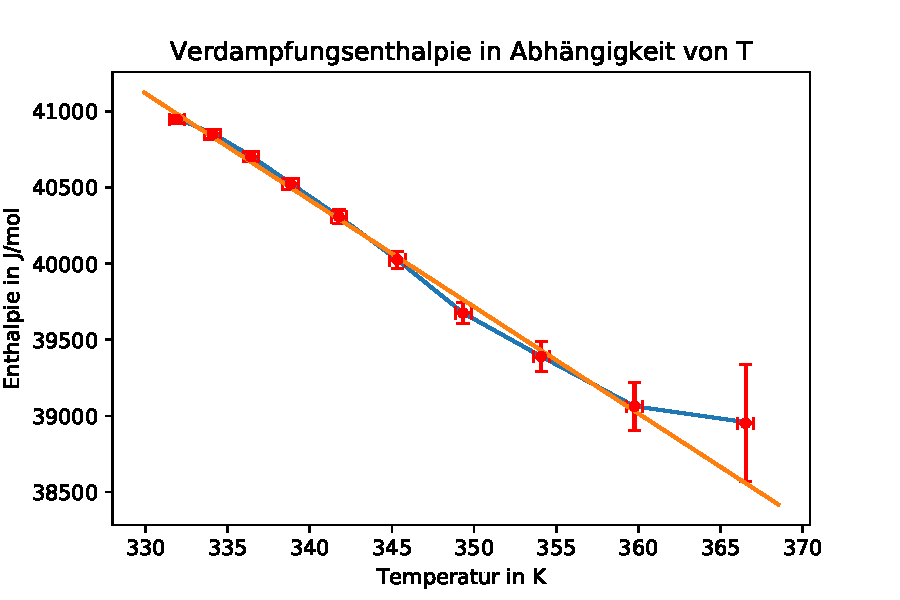
\includegraphics[scale=0.9]{Images/Dampfdruck_L.pdf}
			\caption{Verdampfungsenthalpie $\Lambda$ in Abhängigkeit von der Temperatur}
			\label{DD_L(T)}
		\end{center}
	\end{figure}
	
	\section{Ergebnisse}
	
	\begin{center}
		
		\begin{tabular}{|c|c|}
			\hline
			T in $^\circ$C &  $\Lambda$ in kJ/mol (Literatur)\\
			\hline
			\hline
			40 & 43345.1\\
			\hline
			50  & 42916.1\\
			\hline
			60 & 42478.3\\
			\hline
			70 & 42031.6\\
			\hline
			80 & 41575.8\\
			\hline
			90 & 40873.2\\
			\hline
			100 & 40633.6\\
			\hline  			
		\end{tabular} 
	\end{center}
	Es gibt einige Aspekte, die wir vernachlässigt haben:
	Das genutzte Thermometer hat eine Ansprechzeit von 7s um $99\%$ des wahren Wertes zu erreichen. Das ist zwar oft nicht vernachlässigbar, aber da die Abkühlung sehr langsam vonstatten geht, tritt kein großer Temperaturshift auf.
	Weiterhin ist die Methode, die zur Kalibration des Thermosensors genutzt wurde, zweifelhaft. Bei kochendem Wasser wird die Temperatur vielleicht gut durchmischt sein, sodass man auch einen realen Wert annehmen kann, die Kalibration in Eiswasser aber ist sehr unsicher. Die Temperatur nicht an jeder Stelle gleich, am Eis ist es kälter, am Flüssigkeitsrand durch Wärmeleitung wärmer als die theoretisch angenommenen \SI{0}{\celsius}, sodass man nicht so recht weiß, welchen Fehler man dafür einschätzen soll. Auch bei siedendem Wasser kommt eine Unsicherheit dazu, denn für einen bestimmten Druck herrscht auch eine unterschiedliche Siedetemperatur, die wir an dieser Stelle nicht näher einberechnet haben, da, wie später noch einmal ausgeführt wird, auch der Druck nicht genau bestimmbar ist, und was wieder zu neuen Ablesefehlern geführt hätte.
	Es wäre wahrscheinlich besser gewesen, ohne Kalibrierung zu arbeiten.\\
	Nun zum Druck: Über eine Ungenauigkeit des Drucksensors ist nichts bekannt, auch nicht über seine Funktionsweise. Uns bleibt nur zur Abschätzung die Daten der hiesigen Wetterstation zu berücksichtigen und über die barometrische Höhenformel näherungsweise mit unserer Messung zu vergleichen, wobei allerdings der Luftdruck auch nicht zu messen war. Der Mittelwert unseres Umgebungsdruckes beträgt etwa $\SI{984.8}{\hecto \pascal}$ bei einer Höhe von 279 m ü.NN, die mit Phyphox gemessen wurden. Die Wetterstation gibt zur gleichen Zeit einen Druck von $\SI{991}{\hecto \pascal}$ bei 222 m ü.NN an. Zur Abschätzung: $p(h)=p_0*e^{-\frac{h}{h_B}}$, wobei mit $p_0=\SI{1018}{\hecto \pascal}$ und der barometrischen Höhe $h_B=\SI{8.3}{\kilo \meter}$ gilt: $p(222m) \approx \SI{991}{\hecto \pascal}$ und $p(279m) \approx \SI{984.3}{\hecto \pascal}$. Es sollte also nicht allzu relevante Änderungen geben.\\
	Gravierender dagegen ist die Leckrate des Aufbaus, die zwar herausrechenbar ist, indem man einen exponentiellen Zusammenhang benutzt mit dem von uns bei etwa $0.165*p_0$ gemessenen Anfangswert von etwa $60*(0.010501 \pm 5.3*10^{-5})\SI{}{ \, \milli \bar /{\minute}}$, was aber aus Mangel einer zweiten Dichtigkeitsmessung unterlassen wurde. \\
\end{document}
